%autobuild=true changelog

\documentclass[a4paper,9pt,DIV10,oneside,openany]{scrbook}
\usepackage{index}
\usepackage[onehalfspacing]{setspace}
\usepackage{bibgerm}
\usepackage{tabularx}
\usepackage{bibentry}
\usepackage{ifthen}

% new index for config registry variables
\makeindex
\newindex{ucsConfigRegistry}{ndx}{nnd}{Univention Config Registry-Variablen}

% mini table of contents, we have to redefine text styles used
\usepackage[germanb]{minitoc-hyper}
\def\mtcfont{\small\sf}
\def\mtcSfont{\small\sf}
\def\mtifont{\large\sf}

% new command for chapters
\newcommand{\ucsChapter}[1]{\chapter{#1} \minitoc}

% packages needed in all documents

\usepackage[T1]{fontenc}
\usepackage[utf8]{inputenc}
\usepackage{ngerman}
\usepackage{verbatim}
\usepackage[hyphens,spaces]{url}
\usepackage{listings}
\usepackage{lastpage}
\usepackage{graphicx}
\usepackage{ifthen}
\usepackage{index}
\usepackage{color}
\usepackage{placeins}
\usepackage{float}
\usepackage{longtable}
\usepackage{pifont}
\usepackage{version}
\usepackage{multirow}
\usepackage{eso-pic}
\usepackage{wallpaper}
\usepackage[top=4.5cm, headsep=1.5cm, bottom=3cm, footskip=2cm]{geometry}
%\usepackage{showkeys}  % ENABLE SHOWKEYS TO DISPLAY REFERENCE_TAGS IN DOCUMENT
\usepackage{ucsframed}
\usepackage{marginnote}
\usepackage{placeins}

\def\UrlBreaks{\do\/\do\.\do\-}

\iftrue
% http://www.ctan.org/tex-archive/macros/latex/required/psnfss/psnfss2e.pdf
\usepackage{mathptmx} % roman, formulas
\usepackage{helvet} % sans-serif
\usepackage{courier} % typewriter
\renewcommand{\familydefault}{\sfdefault}
\else
% use font univers as sf-font
\fontfamily{pun}
\selectfont
\sffamily
\renewcommand*{\rmdefault}{pun} % pageheader
\renewcommand*{\sfdefault}{pun} % global font
%\renewcommand*{\ttdefault}{pun} % fixed font, should not be univers
\fi

% Tabbox, can be used to create s.th. like this
%
% ---------------------
% | Tab-Titel         |
% ------------------------------------
% | whatever you want                |
% | and some more of this            |
% ------------------------------------
%
% usage:
%
% \begin{ucsTabbox}{Tab-Titel}
% whatever you want
% and some more of this
% \end{ucsTabbox}

% Tabbox with Info Sign

\newenvironment{ucsInfobox}[1]
{\marginpar{\vspace{3ex}\centering
\includegraphics{abbildungen/info.jpg}}\setlength{\FrameRule}{1pt}\setlength{\fboxsep}{2mm}\begin{ucsframed}{#1}\parskip\baselineskip}
{\end{ucsframed}}

\newenvironment{ucsTabbox}[1]
{\setlength{\FrameRule}{1pt}\setlength{\fboxsep}{2mm}\begin{ucsframed}{#1}\parskip\baselineskip}
{\end{ucsframed}}

\newcommand{\ucsTabentry}[2]{\textbf{#1}\\#2}

%% for the background-image on the title page
%% http://stackoverflow.com/questions/240097/how-to-create-a-background-image-on-titlepage-with-latex
\newcommand\BackgroundPicEven{
\put(0,0){
\parbox[b][\paperheight]{\paperwidth}{%
\vfill
\centering
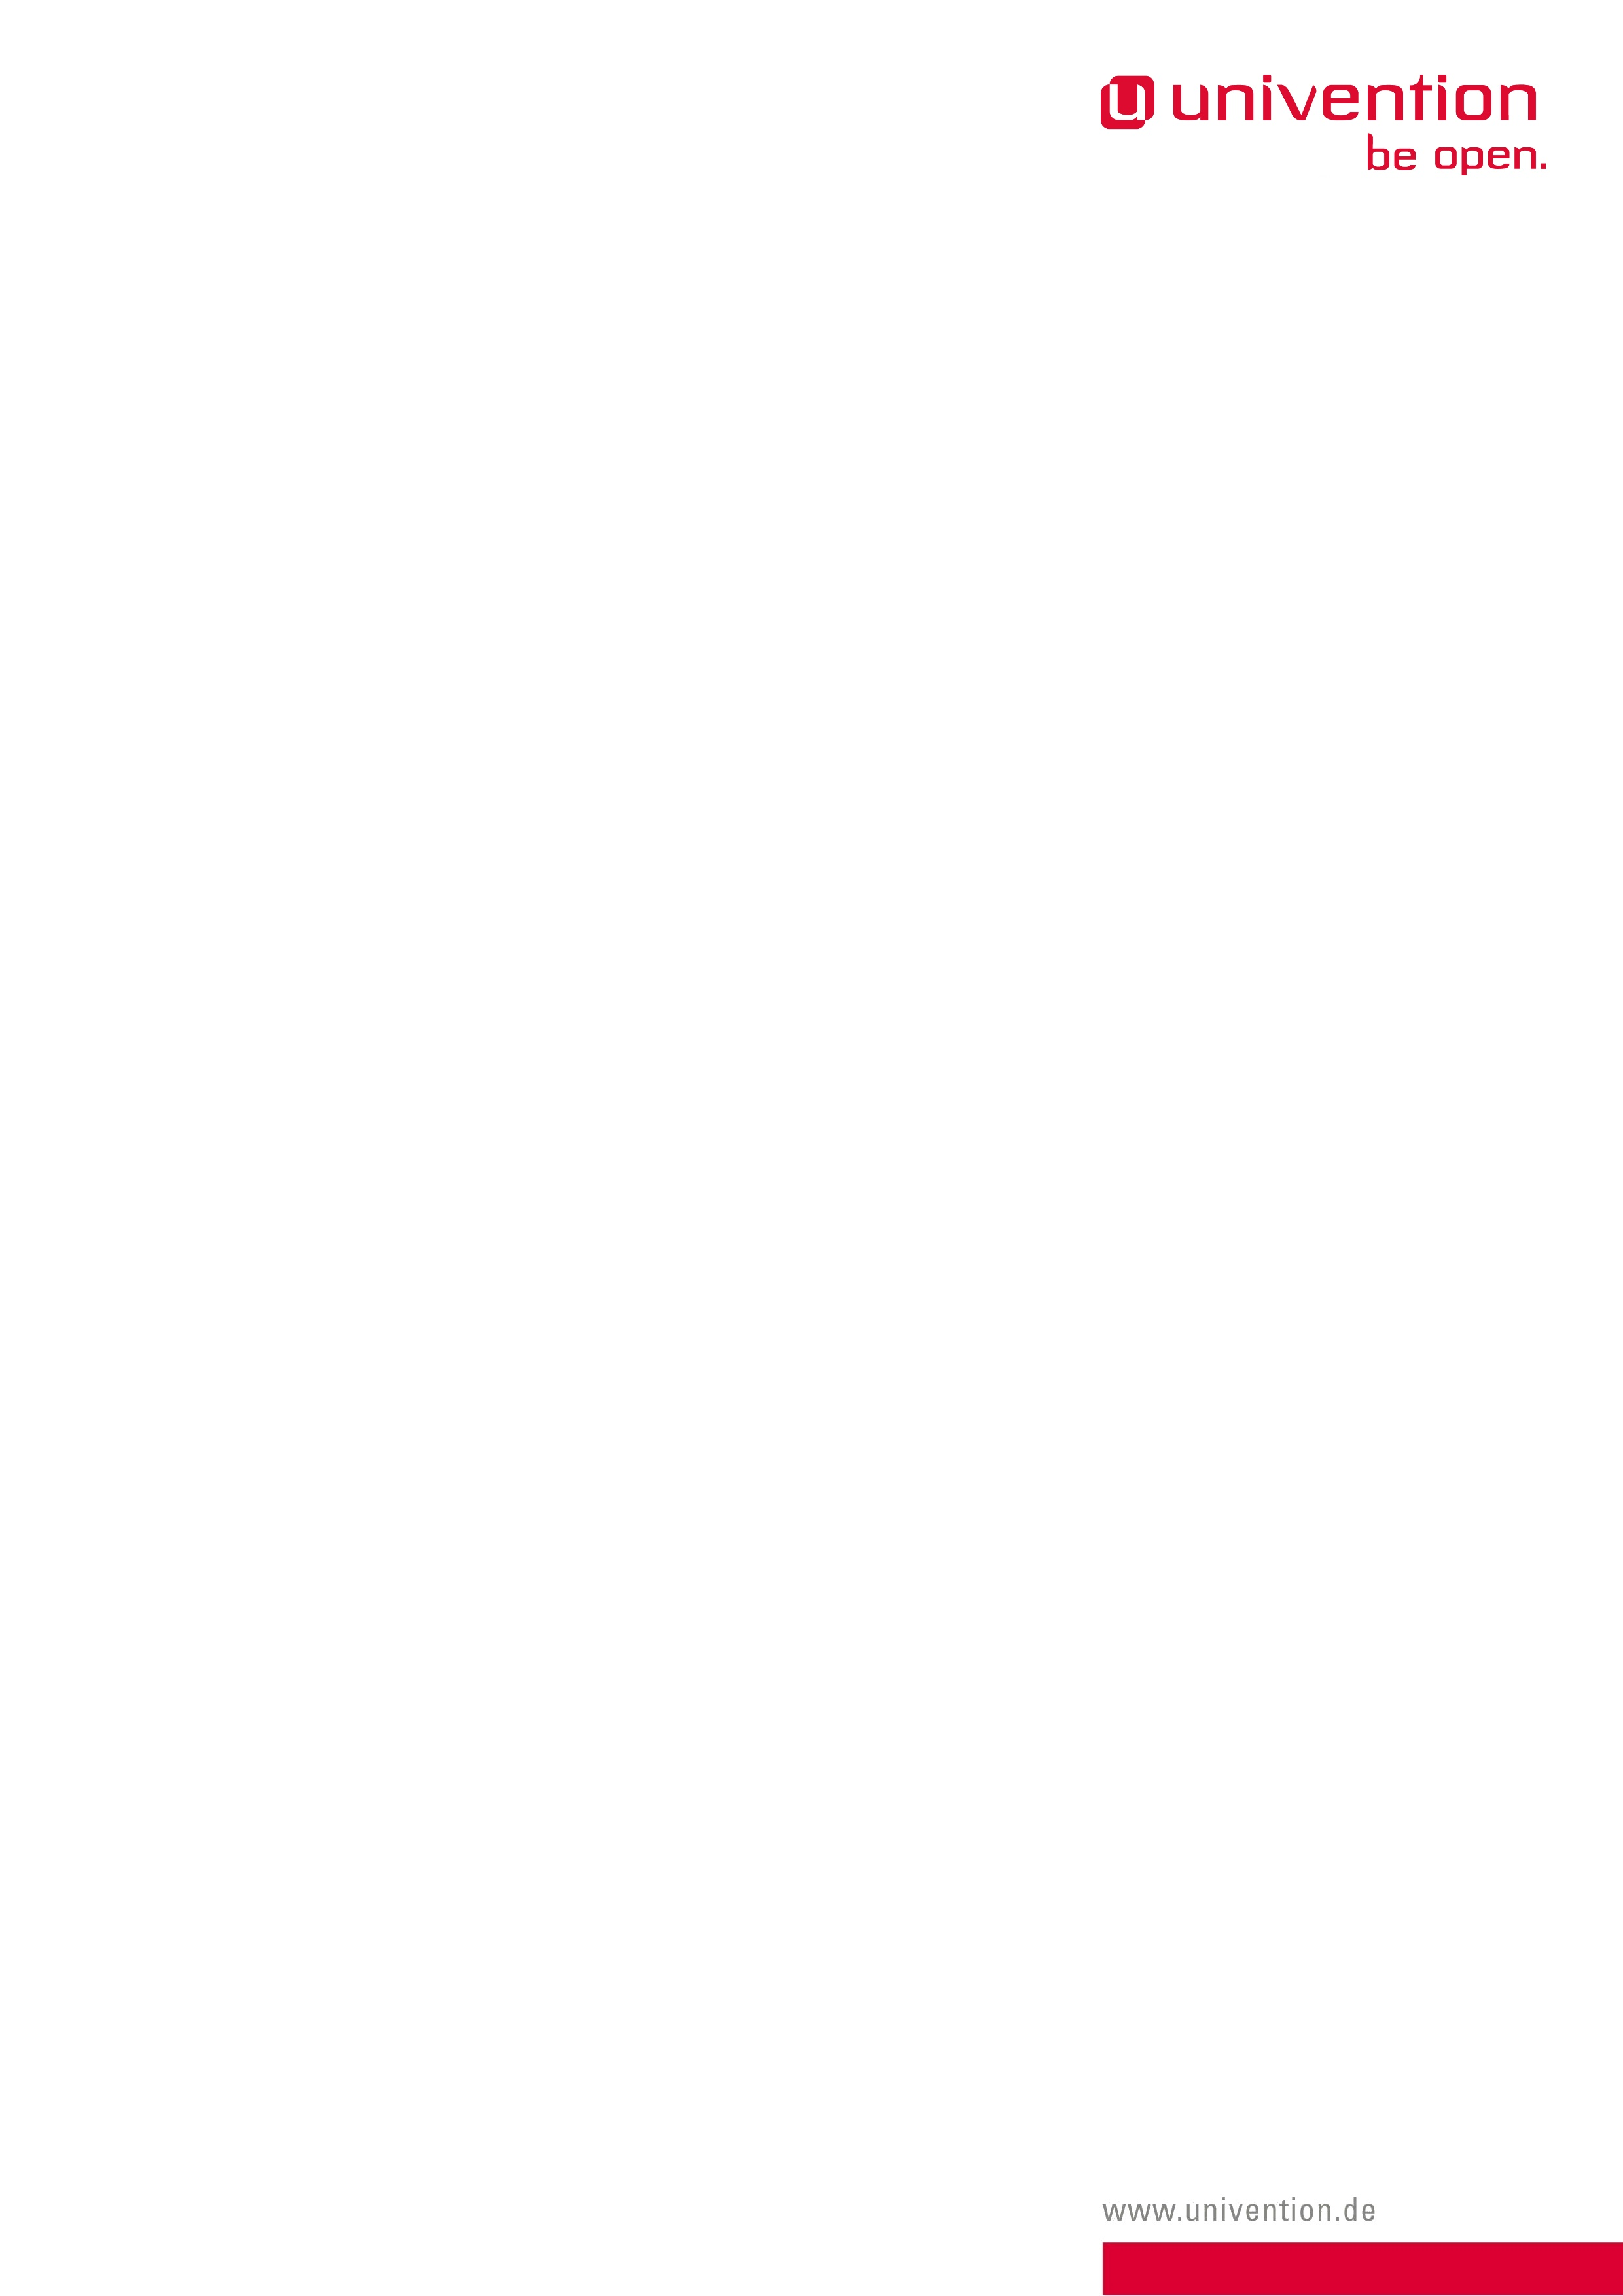
\includegraphics[width=\paperwidth,height=\paperheight]{illustrations/page-background-even.jpg}%
\vfill
}}}

\newcommand\BackgroundPicOdd{
\put(0,0){
\parbox[b][\paperheight]{\paperwidth}{%
\vfill
\centering
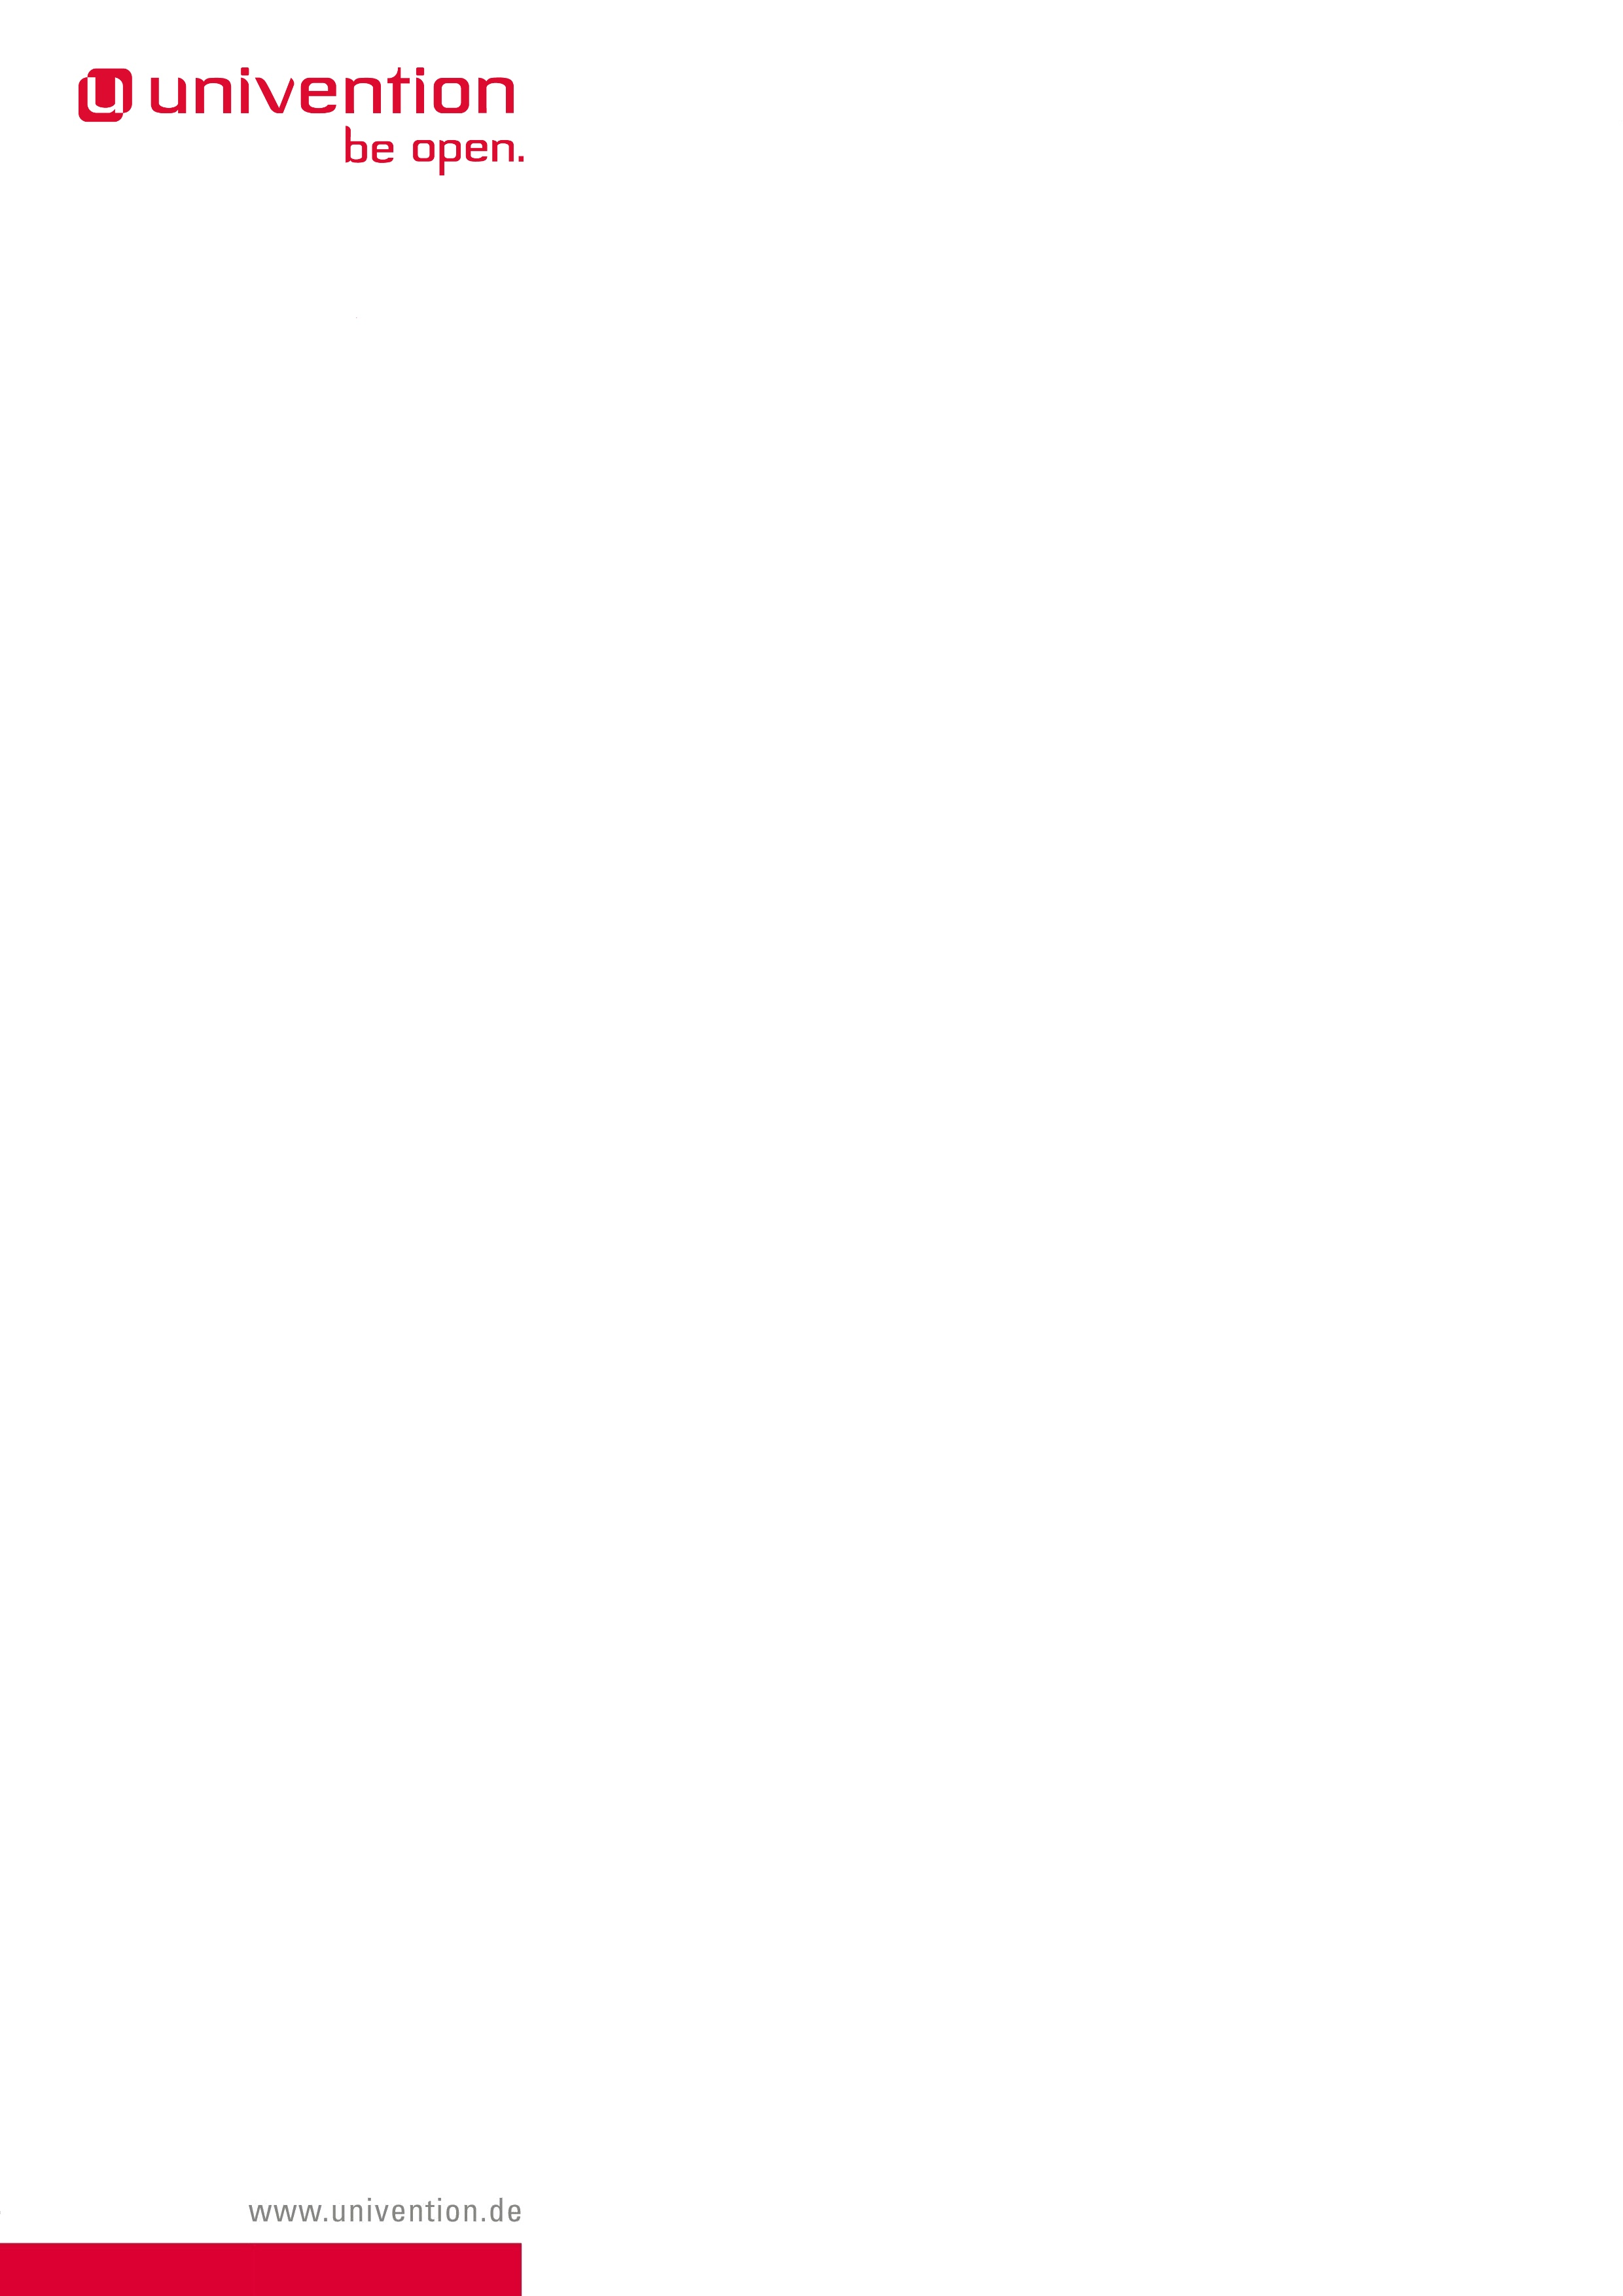
\includegraphics[width=\paperwidth,height=\paperheight]{illustrations/page-background-odd.jpg}%
\vfill
}}}

% Colors:
% red as used in univention corporate identiy
% gray for listing background

\definecolor{ucsRed}{RGB}{0.51372549, 0.141176471, 0.235294118}
\definecolor{ucsCodeGray}{gray}{0.7}
\definecolor{ucsHyperrefLinkColor}{rgb}{0, 0, 0.8}

% tabular environment using sans serif

\newenvironment{tableSansSerif}%
{\begin{table}[H]\footnotesize\sffamily}%
{\end{table}}

% environment for console sessions
\lstnewenvironment{ucsConsoleInput}
 {\lstset{basicstyle=\ttfamily}\small}
 {\normalsize}

% environment for console sessions, boxed
%\lstnewenvironment{ucsConsoleInputBoxed}
% {\lstset{frame=trlb,basicstyle=\ttfamily}\small}
% {\normalsize}

% environment for config files
\lstnewenvironment{ucsConfigFile}
 {\lstset{basicstyle=\ttfamily,backgroundcolor=\color{ucsCodeGray}}\small}
 {\normalsize}

% exclamation mark on border
\newcommand{\ucsExclamation}{\mbox{}\marginnote{\vspace{0pt}\centering\includegraphics{abbildungen/achtung.jpg}}}

% URLs
\newcommand{\ucsURL}[1]{\textsf{\mbox{\url{#1}}}}
%\newcommand{\ucsURL}[1]{\textsf{\url{#1}}}

\newcommand{\ucsFile}[1]{\sloppy{\texttt{#1}}}

% Bugs
\newcommand{\ucsBug}[2][Bug \#]{\href{https://forge.univention.org/bugzilla/show_bug.cgi?id=#2}{#1#2}}

% emphasize text
\renewcommand{\emph}[1]{\textbf{\textsl{#1}}}

% various names
\newcommand{\ucsName}[1]{\sloppy{\textbf{\textsl{#1}}}}

% single command, inline
\newcommand{\ucsCommand}[1]{\sloppy{\texttt{#1}}}

% easy backslash
\newcommand{\BS}{\ensuremath{\backslash}}

% menu entries
\newcommand{\ucsMenuEntry}[1]{\textbf{#1}}

% click buttons
\newcommand{\ucsButton}[1]{\sloppy{[\textbf{#1}]}}

% special notes
\newcommand{\ucsNote}[2][Hinweis:]{\textsl{\textbf{#1}\ifthenelse{\equal{#1}{}}{}{\\}#2}}

% extra note
\newcommand{\ucsAttention}[1]{\textbf{Achtung:}\\#1}

% example
\newcommand{\ucsExample}[2][Beispiel:]{\textbf{#1}\\#2}

% nice right arrow
\newcommand{\ucsRightArrow}{\ding{222}}

% no new paragraph indention
\parindent0cm

% easy integration of bitmaps
\newcommand{\ucsGraphicsTabbox}[3][1]
 {
  \begin{center}
   \includegraphics[width=#1\textwidth]{#3}
   {\refstepcounter{figure}Abbildung \thefigure: \begin{minipage}[t]{0.7\textwidth}{#2}\end{minipage}}
  \end{center}
 }

% easy integration of bitmaps
\newcommand{\ucsGraphics}[3][1]
 {
  \begin{figure}[htb]
  \begin{center}
   \includegraphics[width=#1\textwidth]{#3}
   \ifthenelse{\equal{#2}{}}{}{\caption{#2}}
  \end{center}
  \end{figure}
 }

% easy integration of bitmaps (with reference)
\newcommand{\ucsGraphicsRef}[4][1]
 {
  \begin{figure}[htb]
  \begin{center}
   \includegraphics[width=#1\textwidth]{#3}
   \ifthenelse{\equal{#2}{}}{}{\caption{#2}}
   \label{pic:#4}
  \end{center}
  \end{figure}
 }

% simple index command for univention baseconfig variables
%
% PLEASE do not insert additional spaces or newlines for readability
% they will occur as additional and annoying spaces within final document!
\newcommand{\ucrpath}[1]{% <http://tex.stackexchange.com/questions/50777/>
 \begingroup
 \ttfamily
 \begingroup\lccode`~=`/\lowercase{\endgroup\def~}{/\discretionary{}{}{}}%
 \catcode`/=\active
 \scantokens{#1\noexpand}%
 \endgroup
}
\newcommand{\ucsBCindex}[2][]{\ifthenelse{\equal{#1}{}}{#2}{#1}\index[ucsConfigRegistry]{#2@\ucrpath{#2}}}

\tracingpages=1

% add section number up to subparagraph
\setcounter{secnumdepth}{5}
% add section into index up to subsection
\setcounter{tocdepth}{5}

%wording
\newcommand{\ucsUDM}[1]{Univention Directory Manager#1}
\newcommand{\ucsUDL}[1]{Univention Directory Listener#1}
\newcommand{\ucsUCD}[1]{Univention Corporate Desktop#1}
\newcommand{\ucsUDN}[1]{Univention Directory Notifier#1}
\newcommand{\ucsUMS}[1]{UCS-Managementsystem#1}
\newcommand{\ucsTCS}[1]{Univention Thin Client Services#1}
\newcommand{\ucsUMC}[1]{Univention Management Console#1}
\newcommand{\ucsUCR}[1]{Univention Configuration Registry#1}
\newcommand{\ucsUSS}[1]{Univention System Setup#1}
\newcommand{\ucsUCRV}[1]{\ucsUCR variable \ucsCommand{\ucsBCindex{#1}}}
\newcommand{\ucsUCRVSA}[1]{\ucsCommand{\ucsBCindex{#1}}}
\newcommand{\ucsUAS}[1]{UCS@school#1}
\newcommand{\ucsUVMM}[1]{UCS Virtual Machine Manager#1}

\newcommand{\ucsDVS}[1]{UCS Desktop Virtualization Services#1}
\newcommand{\ucsMaster}[1]{Domänencontroller Master#1}
\newcommand{\ucsBackup}[1]{Domänencontroller Backup#1}
\newcommand{\ucsSlave}[1]{Domänencontroller Slave#1}
\newcommand{\ucsMember}[1]{Memberserver#1}

\newcommand{\ucsUCS}[1]{Univention Corporate Server#1}

\newcommand{\ucsUGS}[1]{Univention Groupware Server#1}
\newcommand{\ucsKolab}[1]{Kolab2 für UCS#1}

%some \ucsUDMb,\ucsUDLCb and \ucsUCRb entrys have to be changed by hand (they do not work in listing environments)
%like  "\begin{ucsConsoleInput}" or something like that
\newcommand{\ucsUCRb}[1]{univention-config-registry#1}
\newcommand{\ucsUDMb}[1]{univention-directory-manager#1}
\newcommand{\ucsUDLCb}[1]{univention-directory-listener-ctrl#1}
\newcommand{\ucsUDNb}[1]{univention-directory-notifier#1}

%not bash but bash style, because there is no command "univention-management-console"
\newcommand{\ucsUMCnb}[1]{univention-management-console#1}



\excludeversion{ucsTech}
\includeversion{ucsDocu}

\usepackage{hyperref}
\hypersetup{ colorlinks,%
             %pdfborderstyle={},% this is what colorlinks defaults to..
             citecolor=ucsHyperrefLinkColor,%
	     filecolor=ucsHyperrefLinkColor,%
	     linkcolor=ucsHyperrefLinkColor,%
	     urlcolor=ucsHyperrefLinkColor%
	   } 

%% Standardschrift: Sans Serif

%% DO NOT CHANGE TO \input{...} !
\input glyphtounicode
\pdfgentounicode=1

\begin{document}

% more spacing between paragraphs
\setlength{\parskip}{1ex plus 0.3ex minus 0.1ex}
\setlength{\oddsidemargin}{0.5cm}
\setlength{\evensidemargin}{0.9cm}

\sffamily



\newcommand{\ucsManualTitle}{UCS@school 3.1 Release Notes}
\newcommand{\ucsManualSubtitle}{Release Notes für die Inbetriebnahme und
Aktualisierung von \ucsUAS{} 3.1}
\newcommand{\ucsManualVersion}{3.1}
\newcommand{\ucsTechAuthor}{ & Univention GmbH & feedback@univention.de}
\newcommand{\ucsSVNVersion}{16319}

\setcounter{secnumdepth}{3}
\setcounter{tocdepth}{3}

%% Titelseite

\begin{titlepage}
  %% Kopf- und Fußzeilen für die Titelseite
  \thispagestyle{empty}

	\ThisLRCornerWallPaper{1.0}{illustrations/page-background-title-page-ucsschool.jpg}

  \vspace*{3cm}
  \sffamily \bfseries
  \begin{center}
    \Huge
      \ucsManualTitle \\ [3.5cm]
    \huge
      \ucsManualSubtitle
  \end{center}
  \normalsize
  \normalfont

\newpage
\AddToShipoutPicture{\ifthenelse{\isodd{\thepage}}%
	{\BackgroundPicOdd}{\BackgroundPicEven}}
\thispagestyle{empty}
\parindent0cm
\sffamily
\vspace*{11cm}

Version \ucsManualVersion \\
Revision \ucsSVNVersion \\
Stand: \today \\
\\
Alle Rechte vorbehalten. / All rights reserved.\\
(c) 2002 bis 2013 \\
Univention GmbH \\
Mary-Somerville-Straße 1 \\
28359 Bremen \\
Deutschland \\
feedback@univention.de \\
\\
Jede aufgeführte Marke und jedes Warenzeichen steht im Eigentum ihrer
jeweiligen eingetragenen Rechtsinhaber. Linux ist ein eingetragenes
Warenzeichen von Linus Torvalds.

The mentioned brand names and registered trademarks are owned by the
respective legal owners in each case. Linux is a registered trademark
of Linus Torvalds.

\end{titlepage}

%% Kopf- und Fußzeilen für den Rest des Dokuments

%% Inhaltsverzeichnis
\dominitoc
\tableofcontents
\newpage



\chapter{Release-Highlights}

Mit Univention Corporate Server 3.1 steht das vierte Release für
\ucsUAS{} zur Verfügung. Es umfasst eine Reihe von Detailverbesserungen und Fehlerkorrekturen sowie die
folgenden Neuerungen:
\begin{itemize}
\item Ein Einrichtungsassistent für UCS@school nach der Installation.
\item Mit dem neuen Release steht die Dokumentation neben dem PDF-Format jetzt auch im HTML-Format zur Verfügung.
\end{itemize}


\section{Aktualisierung auf UCS 3.1}
\ucsUAS{} basiert nun auf UCS 3.1 und profitiert dadurch von allen Erweiterungen und Korrekturen, die direkt
in UCS eingeflossen sind.

\section{Bereitstellung über Univention App Center}
Die Installation von \ucsUAS{} wurde mit der Integration in Univention App Center erheblich vereinfacht.
Mit wenigen Klicks kann im Modul \ucsName{App Center} der \ucsUMC{} \ucsUAS{} auf einem UCS"=System
installiert werden. Die manuelle Anpassung von Repositoryeinstellungen entfällt.

Während des Updates auf UCS 3.1 wird automatisch auf die \ucsUAS{}"=Applikation umgestellt, so
dass weitere Updates über das Univention App Center bezogen werden können.

\section{Einrichtungsassistent für \ucsUAS{}}
Nach der Installation von \ucsUAS{} steht jetzt ein Einrichtungsassistent zur Verfügung, der in wenigen
Schritten alle zur Konfiguration von \ucsUAS{} notwendigen Informationen abfragt und anschließend die
Konfiguration selbstständig vornimmt.

\section{Dokumentation in den Formaten HTML und PDF}
Die Dokumentationen für Administratoren und für Lehrkräfte stehen jetzt nicht nur als PDF sondern auch im
HTML"=Format zur Verfügung. Beide Versionen können unter \ucsURL{http://docs.univention.de/} abgerufen werden.

\chapter{Empfohlene Update-Reihenfolge für Umgebungen mit mehr als einem UCS-Server / Update von Systemen mit UCS-Komponenten}

Für das Update von UCS-Umgebungen mit mehr als einem UCS-System wird
die nachfolgende Vorgehensreihenfolge empfohlen und muss beachtet werden:

Auf dem \ucsMaster{} wird die maßgebliche (authoritative) Version des
LDAP-Verzeichnisdienstes vorgehalten, die an alle übrigen LDAP-Server
der UCS-Domäne repliziert wird. Da bei Release-Updates Veränderungen
an den LDAP-Schemata auftreten können (siehe
Kapitel 3.4.1 des Handbuchs \cite{UCS-Handbuch}) muss der \ucsMaster{} bei einem
Release-Update immer als erstes System aktualisiert werden.
Generell ist es empfehlenswert alle UCS-Systeme möglichst in einem
Wartungsfenster zu aktualisieren. 

\section{Hinweise zu Umgebungen mit Dritt-Software}

Bei der Verwendung von 3rd-Party-Software ist generell \emph{vor} dem Update
mit dem Hersteller/Vertriebspartner der Software zu klären, ob
diese mit der neuen Version von Univention Corporate Server weiterhin
uneingeschränkt einsetzbar ist. 

Die Hersteller/Vertriebspartner von auf Univention Corporate Server
basierenden Produkten sorgen eigenständig für die Veröffentlichung. Updates
müssen daher von dort bezogen werden.

Falls Ihnen von Univention angepasste Paketversionen bereitgestellt wurden, so
sollte geprüft werden, ob durch die Aktualisierung angepasste Pakete
überschrieben werden --- vorzugsweise in einer Testumgebung. Sollten Sie hier
Probleme feststellen, so wenden Sie sich bitte an Univention.

\chapter{Vorbereitung des Updates}
Vor einem Update auf UCS 3.1"=0/\ucsUAS{} 3.1 muss auf UCS 3.0-2 aktualisiert werden.

Es sollte geprüft werden, ob ausreichend Festplattenplatz verfügbar ist. Eine
Standard-Installation benötigt mindestens 6 GB Speicherplatz. Das
Update benötigt je nach Umfang der vorhanden Installation mindestens 2 GB
weiteren Speicherplatz zum Herunterladen und Installieren der Pakete.

Für das Update sollte eine Anmeldung auf der Console mit dem
Benutzer \emph{root} durchgeführt und das Update dort gestartet werden.
Alternativ kann das Update über die \ucsUMC{} durchgeführt werden.

Eine Remote-Aktualisierung über SSH wird nicht empfohlen, da dies
beispielsweise bei Unterbrechung der Netzwerkverbindung zum Abbruch des
Update-Vorgangs und zu einer Beeinträchtigung des Systems führen kann. Sollte
dennoch eine Aktualisierung über eine Netzverbindung durchgeführt werden, ist
sicherzustellen, dass das Update bei Unterbrechung der Netzwerkverbindung trotzdem
weiterläuft. Hierfür können beispielsweise die Tools \ucsCommand{screen} oder
\ucsCommand{at} eingesetzt werden, die auf allen Systemrollen installiert sind.


\chapter{Nachbereitung des Updates}

Nach dem Update sollte auf allen Systemen der
Befehl \ucsCommand{univention-run-join-scripts} als
Benutzer \emph{root} aufgerufen werden, um nicht aufgerufene Joinskripte auszuführen, und
das UCS-System anschließend neu gestartet werden. Alternativ kann die Ausführung 
der Joinskripte auch im UMC"=Modul \ucsName{Domänenbeitritt} ausgelöst werden.

\section{Konfiguration von Freigabeservern je Schule}
Seit \ucsUAS{} 3.1 können an OU"=Objekten im LDAP"=Verzeichnis zwei Fileserver definiert werden.
Sie werden von den Importskripten beim Anlegen von neuen Klassenfreigaben und Heimatverzeichnisfreigaben
ausgelesen und entsprechend an den neuen Freigabeobjekten als Fileserver eingetragen.

Während des Update von \ucsUAS{} 3.0 nach 3.1 werden die zuständigen Fileserver automatisch ermittelt und an
den OU"=Objekten nachgetragen. Es sollten daher die automatisch hinterlegten Fileservereinstellungen aller OUs
überprüft werden. Bei mehreren OUs auf einem Schulserver kann es z.B. sein, dass eine automatische Zuordnung
nicht möglich war. 

Um das automatische Update der OU"=Objekte zu verhindern, kann \emph{vor} dem Update die \ucsUCR{"=Variable} 
\ucsUCRVSA{update31/ucsschool/ou\_fileserver/update} auf dem Domänencontroller Master auf den Wert \emph{no}
gesetzt werden. Die Aktualisierung der OU"=Objekte kann dann nachträglich manuell gestartet werden:\\
\begin{ucsConsoleInput}
root@master# cd /usr/share/ucs-school-import/scripts/
root@master# ./ucs-school-update-ou-fileservers --auto-detect
\end{ucsConsoleInput}


\section{Anpassung der Passwort-Richtlinien beim Einsatz von Samba 4}
Ab UCS 3.1 werden die Einstellungen des Samba-Domänenobjekts (zu
finden im Modul \ucsMenuEntry{LDAP-Verzeichnis} der \ucsUMC{} im Container \emph{samba}) mit den
Samba-Passworteinstellungen synchronisiert. Nach dem Update auf UCS
3.1 greifen dann die strengeren Einstellungen aus Samba 4.

Die Einstellungen sollten nach dem Update geprüft und ggf. angepasst
werden. Hinweise zur Konfiguration finden sich im Kapitel 5.3 des UCS
3.1-Handbuchs (Passwort-Einstellungen für Windows-Clients bei
Verwendung von Samba 4).

Insbesondere wenn bisher kein maximales Passwortalter am Samba-Domänenobjekt gesetzt war,
sollte nach dem Update das maximale Passwortalter in Samba 4 durch
Ausführung des folgenden Kommandos ebenfalls auf den speziellen Wert 0
gesetzt werden:
\begin{ucsConsoleInput}
samba-tool domain passwordsettings set --max-pwd-age 0
\end{ucsConsoleInput}


\section{Anpassung der Dateisystem-Zugriffsrechte für Gruppenrichtlinienobjekte in der Sysvol-Freigabe}
Die in UCS 3.1 eingesetzte Version von Samba 4 verwendet ein
überarbeitetes VFS-Modul zur Speicherung von Dateizugriffsrechten
(NTACLs und fACLs). Nach dem Update sollte der folgende Befehl
einmalig auf allen UCS 3.1 Domänencontrollern mit Samba 4 aufgerufen
werden:
\begin{ucsConsoleInput}
samba-tool ntacl sysvolreset
\end{ucsConsoleInput}
Wegen der Sysvol-Replikation sollte das Kommando als erstes auf dem System aufgerufen werden, das den
Univention S4 Connector bereitstellt, d.h. in den meisten Fällen
zuerst auf dem \ucsMaster{}.



\chapter{Hinweise zum Einsatz einzelner Pakete (siehe auch Release Notes für UCS 3.1)}

\section{Empfohlene Browser für den Zugriff auf die Univention Management Console}

\ucsUMC{} verwendet für die Darstellung der Web-Oberfläche zahlreiche
Javascript- und CSS-Funktionen. Cookies müssen im Browser zugelassen
sein. Die folgenden Browser werden empfohlen:

\begin{itemize}
\item Chrome ab Version 14
\item Firefox ab Version 10
\item Internet Explorer ab Version 9
\item Safari (auf dem iPad 2)
\end{itemize}

Auf älteren Browsern können Darstellungs- oder Performanceprobleme
auftreten.

\section{Aktivierung der Passwortrotation für Samba 4-Domänencontroller}

Die Rotation der Passworte von Samba 4 Domänencontrollern wird beim Update wieder aktiviert.
Dies ist wichtig, weil sich die domänenweite Einstellung für das maximale Passwortalter
unter Samba 4 auch auf Domänencontroller bezieht. Falls die Passswortrotation der
Domänencontroller nicht gewünscht ist, kann sie auf jedem Domänencontroller einzeln
durch Setzen der \ucsUCR{}-Variable \ucsUCRVSA{server/password/change} auf \emph{no} deaktivert werden.

\section{Einschränkungen im Samba 4-Betrieb}

Die aktuell vom Samba-Projekt veröffentlichten Versionen von Samba 4
unterliegen in der Weiterentwicklung noch stärkeren Änderungen als Samba
3. Einige Funktionalitäten stehen daher noch nicht vollständig zur Verfügung:

\begin{itemize}
\item Microsoft Windows Domänencontroller dürfen aktuell nicht in eine Samba 4-Domäne
gejoint werden.
\item Eine selektive Replikation ist mit Samba 4 nicht möglich, da diese durch
Active Directory prinzipiell nicht unterstützt wird (in UCS@school
basiert die selektive Replikation auf der Listener/Notifier-Replikation).
\item Samba 4 unterstützt aktuell keine Forest-Domänen. 
\item Samba 4 unterstützt aktuell keine Vertrauensstellungen.
\end{itemize}

Weitere Hinweise finden sich in Kapitel 8 des UCS-Handbuchs \cite{UCS-Handbuch}.

\section{Deaktivierung der Generierung von LM-Hashes}
In Samba 3 wurden die Passwörter von Benutzern im LM-Hashverfahren gespeichert.
In Umgebungen mit UCS 3.x sind diese Hash-Einträge nicht mehr nötig. 

Ab UCS 3.0 werden keine LM-Hashes mehr generiert. Das alte Verhalten kann durch
Setzen der \ucsUCR{}-Variable \ucsUCRVSA{password/samba/lmhash} auf \emph{true} wieder aktiviert 
werden.



\chapter{Changelog}

Die Changelogs mit den detaillierten Änderungsinformationen werden ab UCS 3.0
nur noch in Englisch gepflegt.

\section{General}
\begin{itemize}
\item Updated copyrights for all packages to 2013 (\ucsBug{30123}).
\end{itemize}

\section{Import scripts}
\begin{itemize}

\item The creation of the incorrect and obsolete userlogon share for
  each school has been removed from the \ucsCommand{create\_ou} import script
  (\ucsBug{15705}).

\item The \ucsCommand{import\_computer} import script now skips computers with an
  existing MAC address instead of generating a new one, which led to
  a traceback when not in district mode (\ucsBug{26446}).

\item The \ucsCommand{import\_user} import script now searches for computers with
  the service \emph{Samba 3} instead of the wrong service name \emph{Samba}
  (\ucsBug{27366}).

\item This update disables the creation of school OUs that contain
  hyphens in their name in order to avoid errors for some UMC modules
  (\ucsBug{27991}).

\item An annoying debug output has been removed (\ucsBug{28324}).

\item The mechanism to determine the correct fileserver for new users \emph{sambaHomePath} has changed. If
  set, the \ucsUCR{} variable \ucsUCRVSA{ucsschool/import/set/sambahome} is used. Otherwise in single server environments the
  domaincontroller master is always used as share fileserver.

  In multi server environments the share fileserver is now read from the corresponding school OU object. The
  fileserver for user home shares will be written automatically into school OU object during OU creation. If
  another fileserver shall be used to create a \emph{sambaHomePath}, OU's fileserver settings may be changed
  via CLI or UMC.

  During the update to UCS@school 3.1 missing fileserver settings at school OU objects will be set
  automatically. Please check the update logfile or the OU objects directly to be sure all settings are
  correct. Especially in environments with multiple school OUs hosted on one school DC all related OU objects
  have to be checked.

  To disable the automatic update of OU's fileserver settings during the update to UCS@school 3.1, the
  UCR variable \ucsUCRVSA{update31/ucsschool/ou\_fileserver/update} has to be set to \emph{no} on domaincontroller master
  before the update is started. The OU update may be manually started afterwards by executing the following
  command (\ucsBug{27549}):\\
  \begin{ucsConsoleInput}
root@master# cd /usr/share/ucs-school-import/scripts/
root@master# ./ucs-school-update-ou-fileservers --auto-detect
  \end{ucsConsoleInput}

\item The command \ucsCommand{move\_domaincontroller\_to\_ou} has been added to move domaincontroller slave
  objects to a specified school OU if the object has been created e.g. in the global computer container. It
  keeps track of e.g. the share file server settings at school OU objects and changes them accordingly (\ucsBug{27242}).

\end{itemize}

\section{iTALC}
%\begin{itemize}
%
%\end{itemize}

\section{Domain services}

% \subsection{OpenLDAP}
% \begin{itemize}
% \end{itemize}

\subsection{LDAP ACL changes}
\begin{itemize}
\item The LDAP subtree below \emph{cn=license,cn=univention,BASEDN} can now be replicated by UCS@school
  domaincontroller slave systems. This change is required for proper use of Univention App Center
  (\ucsBug{30229}).
\end{itemize}

\subsection{LDAP schema changes}
\begin{itemize}
\item The UCS@school LDAP schemata has been updated by removing some unused comments (\ucsBug{20663}).
\end{itemize}

% \subsection{Listener/Notifier domain replication}
% \begin{itemize}
% \end{itemize}

\subsection{Domain joins of UCS systems}
\begin{itemize}
\item A new join script has been added which will only be executed on a DC
  slave. This script will check if the DC slave's computer object is at the
  right place inside the LDAP tree as well as verify the permissions
  (\ucsBug{26834}).
\end{itemize}

\subsection{Services for Windows}
\begin{itemize}
\item A traceback during directory creation in the \ucsUDL{ module} \ucsName{ucs-school-user-logonscripts.py}
  has been fixed (\ucsBug{28121}).
\item Due to an offline caching related bug in Windows XP, the netlogon script based assignment of
  \ucsName{My documents} / \ucsName{Eigene Dateien} and \ucsName{My pictures} / \ucsName{Eigene Bilder} to
  the server stored home directory leads to permission problems during user logoff.
  By default the assigment is now deactivated for new users and can be reactivated by setting the
  UCR variable \ucsUCRVSA{ucsschool/userlogon/myshares/enabled} to \emph{yes} on the master domain controller and (if
  existing) slave domain controllers.

  After changing the UCR variable, a resync of the Univention Directory Listener module 
  \emph{ucs-school-netlogon-user-logonscript} is advised to update the user logonscripts and recreate missing logon
  scripts (\ucsBug{28214}).
\item The permissions of the netlogon script \ucsCommand{ucs-school-logon.vbs} will be now set to 0644 on each
  change. Additionally the owner will be set to root:root (\ucsBug{30284}).
\item The listener module \ucsName{ucs-school-user-logonscript} now respects the following two \ucsUCR{}
  variables defining the output directory for new logon scripts:
  \begin{itemize}
  \item \ucsCommand{ucsschool/userlogon/netlogon/path}
  \item \ucsCommand{samba/share/netlogon/path}
  \end{itemize}
  The first mentioned variable has higher priority (\ucsBug{28205}).
\item The filename for the listener module \ucsFile{ucs-school-user-logonscripts.py} has been renamed to
  \ucsFile{ucs-school-user-logonscript.py} to match to the listener modules internal name (\ucsBug{28452}).

\item The DNS SRV record mapping for the S4 connector will be
preconfigured with this release. This is required for the Samba 3 to
Samba 4 migration (\ucsBug{27395}).

\item The UCR variables \ucsName{dns/register/srv\_records/gc},
\ucsName{dns/register/srv\_records/pdc} and
\ucsName{samba4/dns/domain/register} will be set to \ucsName{false} on a
school slave installation and upgrade. This prevents the SRV registration for
GC and PDC records and the IP registration at the forward zone. Thus the
overwriting of the DNS SRV records on the master has been removed
(\ucsBug{28754}).

\item SRV record priority and weight were permuted in the ucs-school-slave S4 connector DNS mapping overrides.
While probably a cosmetic issue, this is now fixed for slaves joining with the new release (\ucsBug{30166}).

\item The DNS service account is now created in a separate join script \ucsName{univention-samba4-slavepdc}
to avoid a conflict with \ucsName{libunivention-ldb-modules} (\ucsBug{30105}).

\item \ucsName{ucs-school-slave} now sets the UCR variables \ucsUCRVSA{samba4/ignore/mixsetup} and
  \ucsUCRVSA{samba3/ignore/mixsetup} to \emph{yes} during initial installations of the package to facilitate
  migration scenarios and deployment by the new installation wizard (\ucsBug{30212}, \ucsBug{30302}).

\item Initialize UCR variable \ucsUCRVSA{windows/wins-support} before running the joinscript of \ucsName{univention-samba} (\ucsBug{30267}).
\end{itemize}

%\subsection{Univention S4 Connector}
%\begin{itemize}
%
%\end{itemize}

% \section{Print services}
% \begin{itemize}
% \end{itemize}

%\section{Proxy services}
%\begin{itemize}
%
%\end{itemize}

%\section{RADIUS}
%\begin{itemize}
%\end{itemize}

%\section{Univention Directory Manager modules}
%\begin{itemize}
%
%\end{itemize}

\section{Univention Management Console}

%\subsection{Univention Management Console server}
%\begin{itemize}
%
%\end{itemize}

%\subsection{Univention Management Console web interface}
%\begin{itemize}
%
%\end{itemize}

\subsection{Univention Management Console modules}
\begin{itemize}

\item All UMC modules have been ported to the new version of the Dojo toolkit
  (\ucsBug{29793}, \ucsBug{29787}, \ucsBug{29792},
  \ucsBug{29791}, \ucsBug{29790}, \ucsBug{29784}, \ucsBug{29788},
  \ucsBug{29786}, \ucsBug{29785}, \ucsBug{29789}, \ucsBug{29776}).

\item A new module to guide the initial configuration of UCS@school in a domain has
been added (\ucsBug{30162}).

\item This update disables the creation of school OUs that contain
  hyphens in their name in order to avoid errors for some UMC modules
  (\ucsBug{27991}).

\item Added missing scrollbars for the detail view of UMC modules
  \ucsName{Room management}, \ucsName{Assign teachers to classes},
  \ucsName{Administrate workgroups} (\ucsBug{27941}).

\item Corrected the behaviour when cancelling the delete action in the confirmation dialog (\ucsBug{28213}).

\item Shares are now automatically created and removed along with workgroups (\ucsBug{28211}).

\item Assigning internet rules failed when /dev/squid/ and /var/lib/ucs-school-webproxy/ resided on different partitions (\ucsBug{29891}).

\item Old greylist internetrules from UCS 2.4 does not produce a traceback anymore (\ucsBug{28684}).

\item Fix initial search query on assign page in \ucsName{internetrules} module (\ucsBug{27726}).

\item Fix encoding of ucr keys which leads to traceback when assigning internetrules (\ucsBug{29948}).
\item Remove duplicated error messages (\ucsBug{27940}).
\item Use new template method for help page (\ucsBug{27681}).
\item Display a more detailed error message if the IP or MAC address is
  already in use in the computer wizard (\ucsBug{27393}).
\item The ''lock'' option in the computerroom module has been renamed into ''lock screen''. Also fixed a little typo in german translation (\ucsBug{27246}).
\item If connection to a computer room is lost, the module tries to reconnect
  five times before giving up and displaying an error message. This is done
  because of segfaults caused by iTalc not yet fully understood
  (\ucsBug{27202}).
\item The computerroom module checks if VNC received a screenshots of the
  requested computer before sending it. This does not change the behaviour of
  the module, but it prevents ``silent'' tracebacks in the log files of that
  module (\ucsBug{28674}).
\item Fixed some little issues in MultiUploader (\ucsBug{28818}).
\item In some cases groups without the prefix ''<schoolname>-'' would not be
  displayed (\ucsBug{29830}).
\item Teachers are no longer added to a class automatically. After a user is
  created, the first widget on the page will be focussed (\ucsBug{27954}).
\item The password module now respects the
  UCR variable \ucsUCRVSA{directory/manager/web/modules/autosearch} option (\ucsBug{28200}).
\item The list of school OUs is now updated at each request. This avoids the
  necessity to relogin after creating a new school OU (\ucsBug{30046}).

\item In the wizards module the password of a user will be validated before
  creating the user object (\ucsBug{30091}).

\item A typo in the password module has been corrected (\ucsBug{30134}).

\item Hyphens have been enabled for the name of slave DC in the wizard
  ``Add school'' (\ucsBug{30232}).

\end{itemize}

\section{Other changes}
\begin{itemize}
\item During the update to UCS@school 3.1 the repository configuration will be altered automatically.
  Further release updates of UCS@school have to be installed via Univention App Center (\ucsBug{30221}).
\end{itemize}


\newpage
% \bibliographystyle{gerplain}
\bibliographystyle{unsrt}
\bibliography{referenzen}


\end{document}
